\documentclass[a4paper,12pt]{article}
\usepackage[utf8]{inputenc}
\usepackage[french]{babel}
\usepackage{graphicx}
\usepackage{palatino}
\usepackage[T1]{fontenc}
\usepackage{listings}
\usepackage{color}
\usepackage{float}
\usepackage{amsthm}

\lstset{
  basicstyle=\footnotesize,
  breakatwhitespace=true,
  breaklines=true,
  frame=single,
  keepspaces=true,
  keywordstyle=\color{blue},
  language=Python,
}

\newcommand{\code}[1]{\texttt{#1}}

\begin{document}
\makeatletter
\def\clap#1{\hbox to 0pt{\hss #1\hss}}%
\def\ligne#1{%
\hbox to \hsize{%
\vbox{\centering #1}}}%
\def\haut#1#2#3{%
\hbox to \hsize{%
\rlap{\vtop{\raggedright #1}}%
\hss
\clap{\vtop{\centering #2}}%
\hss
\llap{\vtop{\raggedleft #3}}}}%
\def\bas#1#2#3{%
\hbox to \hsize{%
\rlap{\vbox{\raggedright #1}}%
\hss
\clap{\vbox{\centering #2}}%
\hss
\llap{\vbox{\raggedleft #3}}}}%

\def\maketitle{%
\thispagestyle{empty}\vbox to \vsize{%
\haut{}{\@blurb}{}
\vfill
\vspace{1cm}
\begin{flushleft}
\usefont{OT1}{ptm}{m}{n}
\huge \@title
\end{flushleft}
\hrule height 4pt
\begin{flushright}
\usefont{OT1}{phv}{m}{n}
\large \@author
\end{flushright}
\begin{flushleft}
\end{flushleft}
\vspace{1cm}
\vfill
\begin{center}

\includegraphics[width=.5\textwidth]{./pix/logo.png}
\end{center}
\vfill
\vfill
\bas{}{\@location, le \@date}{}
}%
\cleardoublepage
}
\def\date#1{\def\@date{#1}}
\def\author#1{\def\@author{#1}}
\def\title#1{\def\@title{#1}}
\def\location#1{\def\@location{#1}}
\def\blurb#1{\def\@blurb{#1}}
\makeatother

\title{Intelligence artificielle pour un Force 3\\ \large Rapport de projet}
\author{Julien \textsc{Voisin} \\ Tao \textsc{sauvage} \\ Robin \textsc{Faury}}
\location{Belfort}
\blurb{%
Rapport de projet d'IA41\\
Université de Technologie de Belfort-Montbeliard
}


\maketitle
\newpage

\tableofcontents
\newpage

\section*{Introduction}
Ce document présente le jeu de Force 3 (et plus particulièrement son intelligence artificielle) réalisé dans le cadre de l'UV d'IA41 en langage Prolog.

\section{Règles du jeu}
Édité par \emph{Ravensburger} à partir de 1982, le \emph{force 3} est un mélange entre un jeu de taquin et un tic-tac-toe. Le plateau de jeu est constitué de 3 lignes et 3 colonnes (soit 9 cases en tout). En début de partie, le taquet est placé au centre, et les joueurs placent tour à tour leurs pions. Une fois leurs pions placés, les joueurs peuvent les déplacer.

\subsection{Mécanismes}
Chaque joueur effectue à tour de rôle l'un des trois mouvements suivants:
\begin{enumerate}
	\item Poser un disque de sa couleur sur un carré inoccupé.
	\item Déplacer un carré par glissement, occupé ou non par un pion. Si l'emplacement libre du tablier se trouve sur un bord, il est possible de déplacer deux carrés en un seul coup. Cependant, le joueur peut choisir d'en déplacer un seul.\\
	 Au tour suivant, il n'est pas possible de remettre les carrés dans leur position précédente. Si un joueur fait glisser deux carrés, au coup suivant son adversaire pourra déplacer l'un de ces carrés puisque la position précédente ne sera pas reconstituée.
    \item Déplacer l'un de ses disques, déjà en place sur un carré, vers n'importe quel autre carré inoccupé.
\end{enumerate}
    
\subsection{Victoire}
La partie est gagnée quand un joueur réussi à aligner verticalement, horizontalement ou en diagonale ses trois pions.
\clearpage

\section{Analyse}
\subsection{Estimation du nombre de plateaux possibles par partie}
A partir d'un plateau $p_0$, il est possible (en général) de faire:
\begin{itemize}
	\item 6 déplacements
	\item 8 glissements
\end{itemize}

Soit une petite quinzaine de mouvements (sans compter la phase de placements de pions). Une partie semble durer en moyenne aux alentours de 20 coups. Ce qui nous amène à environ $15^{15}$ coups possibles pour une seule partie.\\

Bien qu'étant une estimation \emph{à la louche}, $15^{15}$ coups sont impossibles à calculer, et à stocker sur des machines actuelles. Une approche par dénombrement n'est donc pas envisageable.

\subsection{Observations}
\begin{itemize}
	\item Le \emph{Force 3} est un jeu à somme nulle (La somme des gains des deux joueurs est nulle).
	\item Il ne faut pas seulement chercher à gagner, il faut également éviter que l'adversaire ne gagne avant nous.
\end{itemize}

\newpage

\section{Formalisation et méthode de résolution}
Au vue des observations précédentes, nous avons choisi d'utiliser un algorithme MiniMax (vu en cour), dans sa variante NégaMax, accompagné d'un élagage $\alpha\beta$.
\begin{figure}[h]
    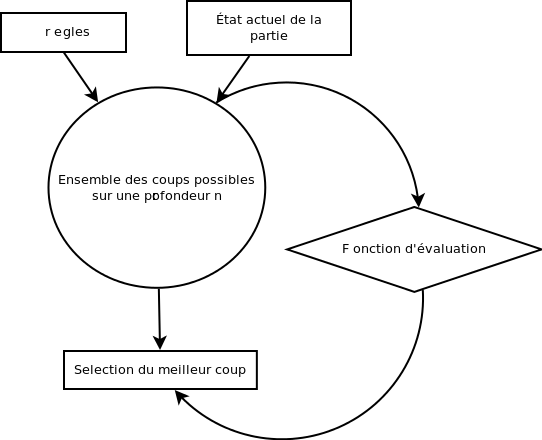
\includegraphics[width=0.8\textwidth]{./pix/methode.png}
    \centering
    \caption{Solution retenue}
\end{figure}

\subsection{Fonction d'évaluation}
\subsubsection{Attribution des points}
Un plateau est constitué de 3 \emph{lignes} verticales, 3 \emph{lignes} horizontales et de 2 lignes \emph{diagonales}. La fonction d'évaluation assigne un score par ligne en fonction du nombre de pions qui y sont présents:
\vspace{1em} % hack
\begin{itemize}
	\item Un pion : 1 point
	\item Deux pions: 5 points
	\item Trois pions : 100 points.
\end{itemize}
\vspace{1em} % hack
Le fait d'affecter une valeur supérieure au double de points donnés à un seul pion, pour deux pions alignés, permet de privilégier ce dernier cas. De plus, attribuer 100 points lorsque trois pions sont alignés l'influencera fortement l'algorithme à tendre vers la victoire !

\subsubsection{Objectifs de convergence}
Cette fonction d'évaluation aura non-seulement tendance à favoriser l'alignement de pions, mais également les positions \emph{stratégiques}, offrant un grand nombre de possibilités de jeu, comme le centre ou les angles.
\begin{itemize}
	\item Un angle est à la fois contenu sur une ligne, une colonne, et une diagonale. Il rapportera donc au minimum 3 points.
	\item Le centre est à la fois contenu sur une ligne, une colonne, et deux diagonales. Il rapportera donc au minimum 4 points.
\end{itemize}

\subsubsection{Exemple d'évaluation d'un plateau}
\begin{figure}[h!]
    \centering
    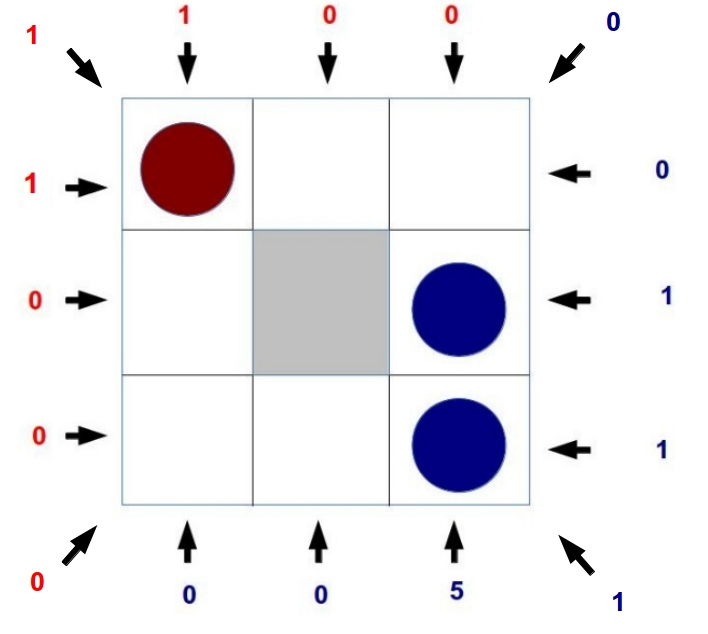
\includegraphics[width=.6\textwidth]{./pix/evaluation.jpg}
    \caption{Exemple de calcul de la fonction d'évaluation}
\end{figure}
\begin{itemize}
	\item Score du joueur rouge: $1 + 1 + 1 = 3$
	\item Score du joueur bleu: $5 + 1 + 1 + 1 = 8$
	\item Évaluation pour le joueur rouge: $3 - 8 = -5$
	\item Évaluation pour le joueur bleu: $8 - 3 = 5$
\end{itemize}


\subsection{Algorithme MiniMax}
\subsubsection{Principe}
Le principe de l'algorithme MiniMax est relativement simple :
\begin{enumerate}
\item Détermination de la liste des coups possibles par le joueur courant.
\item Pour chaque coup, détermination de la liste des coups possibles par l'adversaire.
\item Répétition des deux points précédents jusqu'à la profondeur $n$ définie par l'heuristique.
\item Évaluation des plateaux obtenus.
\item Ces valeurs sont remontées dans les n\oe{}uds de l'arbre de recherche, en sélectionnant le maximum quand c'est un tour du joueur courant, et du minimum si c'est son adversaire.
\item Finalement, choix de la meilleure branche possible pour le joueur courant.
\end{enumerate}

\subsubsection{Négamax}
Le fait que le \emph{Force 3} soit un jeu à somme nulle permet d'utiliser la variante \emph{Négamax} du MiniMax, permettant une implémentation simplifiée en posant :

\begin{figure}[H]
    \code{max(a, b) == -min(-a, -b)}
    \centering
    \caption{Simplification}
\end{figure}
  
\subsubsection{Pseudo-Codes}
\begin{figure}[H]
\centering
\begin{lstlisting}
int maxi( int depth ) {
  int max = -oo;
  if ( depth == 0 )
    return evaluate();
  for ( all moves) {
    score = mini( depth - 1 );
    if( score > max )
      max = score;
  }
  return max;
}
 
int mini( int depth ) {
  int min = +oo;
  if ( depth == 0 )
    return -evaluate();
  for ( all moves) {
    score = maxi( depth - 1 );
    if( score < min )
      min = score;
  }
  return min;
}
\end{lstlisting}
\caption{Pseudo-code simplifié de l'algorithme du MiniMax}
\end{figure}
\begin{figure}[H]
\centering
\begin{lstlisting}
int negaMax( int depth ) {
  int max = -oo;
  
  if ( depth == 0 )
    return evaluate();
    
  for ( all moves)  {
    score = -negaMax( depth - 1 );
    if( score > max )
      max = score;
  }
  return max;
}
\end{lstlisting}
\caption{Pseudo-code simplifié de l'algorithme du Négamax}
\end{figure}
  
\subsubsection{Élagage Alpha/Beta}
Un des soucis d'un tel algorithme est qu'il \emph{requiert beaucoup de place}. En effet, il va parcourir toutes les branches de l'arbre de recherche, alors que ça n'est pas forcément nécessaire. On peut l'optimiser à l'aide d'un élagage de type $\alpha\beta$ (Alpha/Beta), qui permet de réduire de manière conséquente le nombre de n\oe{}ds parcourus, sans pour autant changer quoi que ce soit au résultat final.
\\\\
Sur la figure 6 on peut constater que certaines branches sont superflues. Par exemple, le n\oe{}d de profondeur 1 à droite (5) va prendre la valeur minimum de ses fils. Sachant qu'un 5 est présent, on peut se permettre d'élaguer la branche de droite à partir du n\oe{}ud 8, de profondeur 2, puisque 5 est inférieur à 8.

\subsection{Exemple}
\begin{figure}[H]
    \centering
    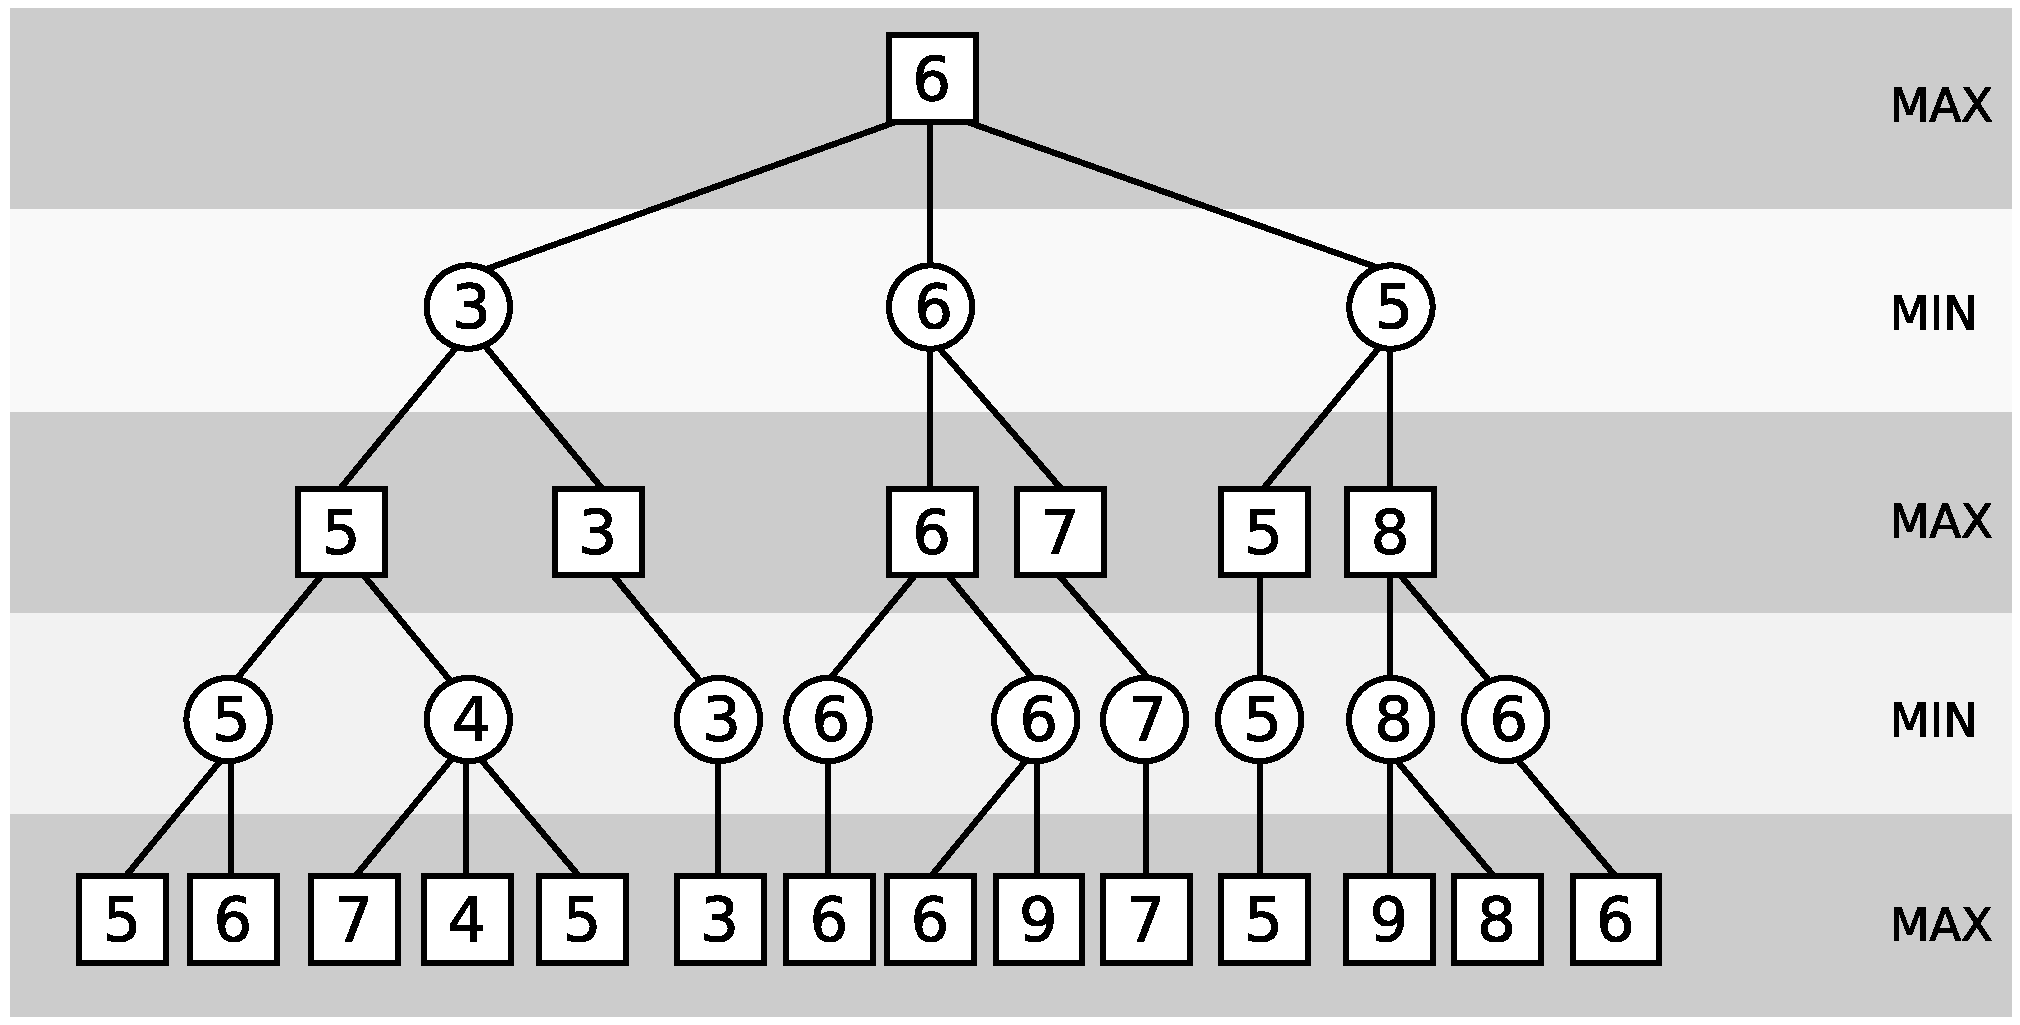
\includegraphics[width=.8\textwidth]{./pix/minimax}
    \caption{Min-max sans élagage}
\end{figure}

\begin{figure}[H]
    \centering
    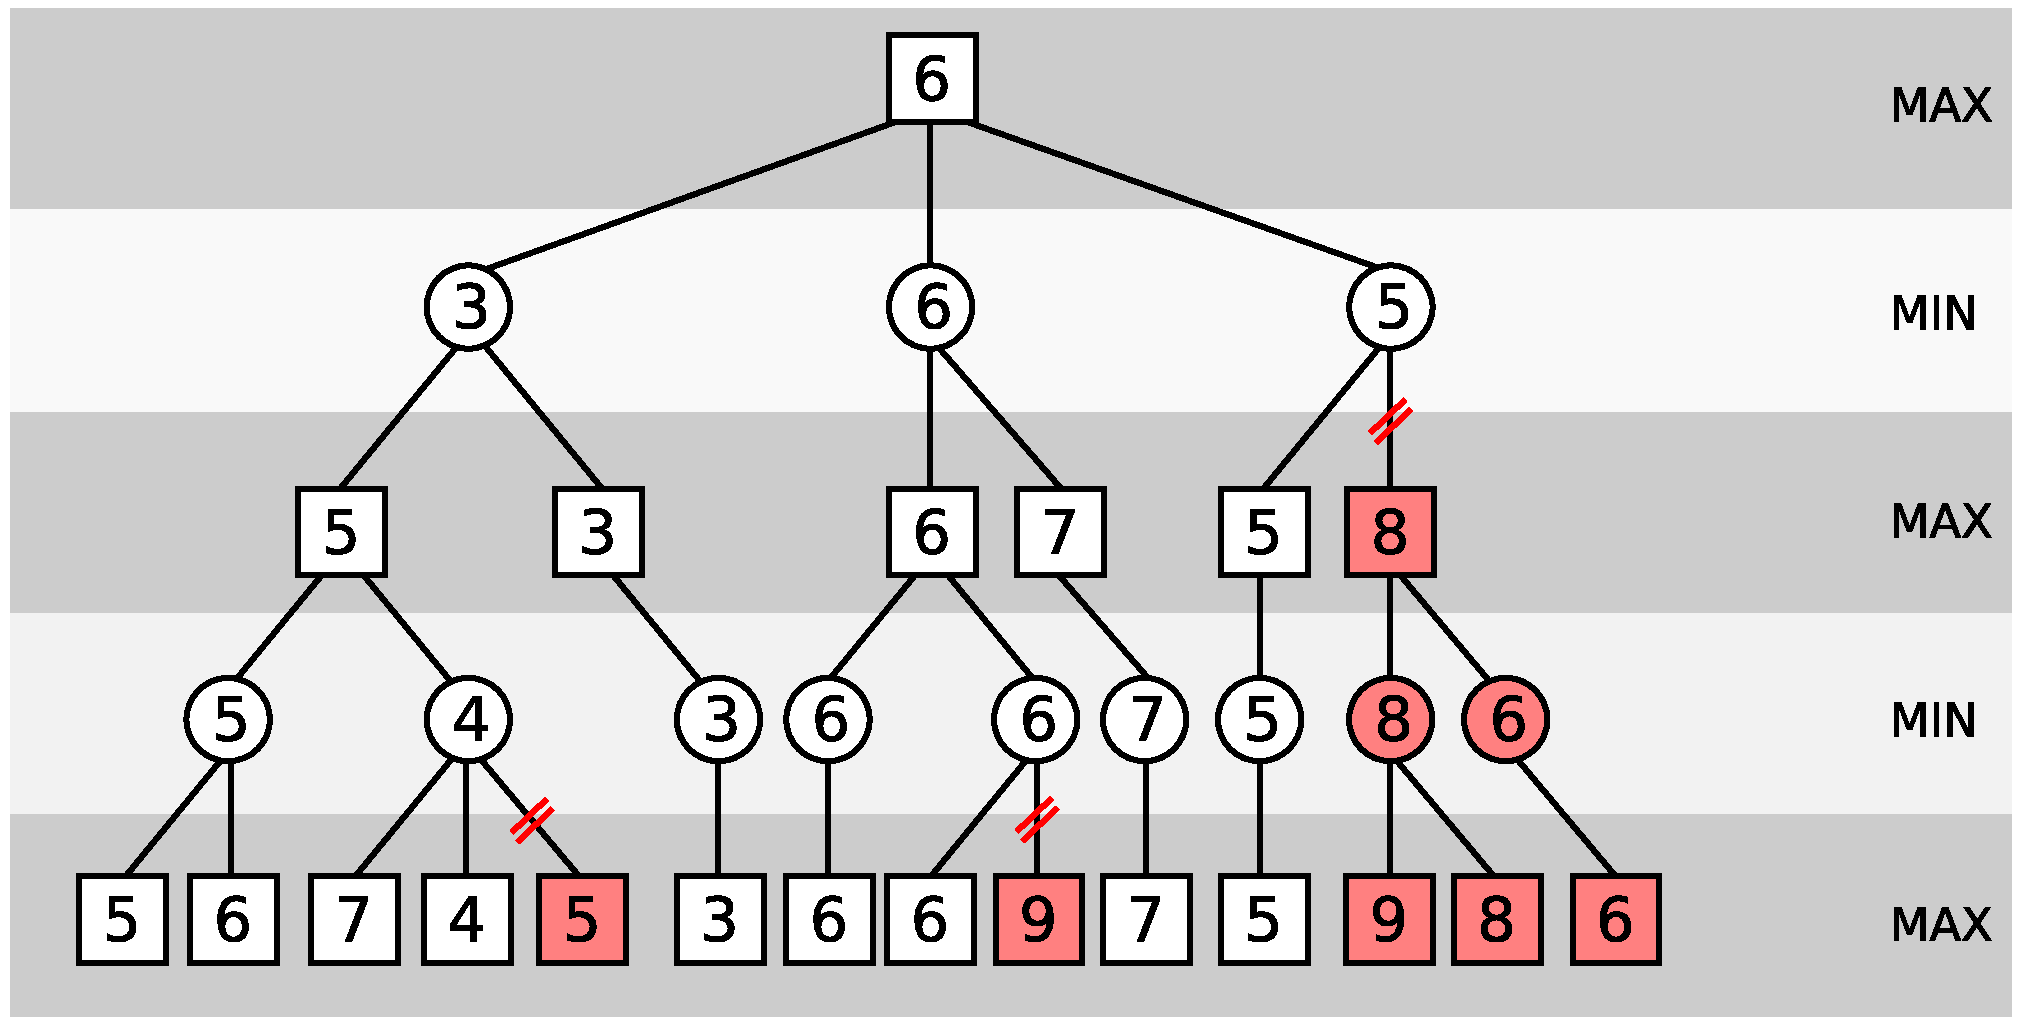
\includegraphics[width=.8\textwidth]{./pix/alphabeta}
    \caption{Min-max avec élagage $\alpha\beta$}
\end{figure}
\newpage

\section{Implémentation}
Cette partie présente les choix d'implémentations, comme la représentation des données, l'interface utilisateur,
la traduction des règles en Prolog, \dots

\subsection{Compatibilité}
Le projet utilise des prédicats spécifiques a SWI-Prolog, et n'a été testé que sur des versions supérieures à la 5.10. Il pourrait donc de pas marcher sur des versions précédentes.

\subsection{Organisation des fichiers}
Le \emph{Makefile} fourni permet de compiler le programme (action par défaut) et de le lancer (\emph{make play}). Le projet est découpé en 5 fichiers:
  \begin{itemize}
    \item \textbf{evaluation.pl} Fonction d'évaluation et algorithme NégaMax avec élagage Alpha/Beta
    \item \textbf{gui.pl} Interface utilisateur, autant affichage qu'interactions.
    \item \textbf{jeu.pl} Prédicats des coups.
    \item \textbf{regles.pl} Règles du jeu et conditions de victoire.
    \item \textbf{main.pl} Permet de lancer le jeu.
  \end{itemize}

\subsection{Représentation des données}
\subsubsection{Plateau}
Le plateau est une grille de $3 * 3$ cases, dont l'emplacement central est \emph{vide} en début de partie.
Le grille est donc représentée comme une liste de 9 éléments pouvant être:
  \begin{description}
    \item[0]  Case vide
    \item[1]  Case portant un pion du joueur 1
    \item[2]  Case portant un pion du joueur 2
    \item[-1] Case taquin
  \end{description}
  
  \begin{figure}[h]
    \code{[1,0,1,-1,0,0,2,1,0]}
    \centering
    \caption{Exemple de plateau}
  \end{figure}
  
Le plateau initial est instancié ainsi:\\
  \begin{figure}[h]
\code{plateau\_vide([0,0,0,0,-1,0,0,0,0]).}
    \centering
    \caption{Plateau initial}
  \end{figure}

\subsubsection{Coup}
Les règles du Force 3 ont été transcrites en un seul prédicat : \textbf{deplacement/3 (+Joueur, +Plateau, -[Case1, Case2, IdMouvement])}. Il définit les conditions particulières associées à chaque type de coup (pose d'un pion, déplacement d'un pion, déplacement d'une case, déplacement de deux cases).

Ce prédicat est ensuite utilisé dans \texttt{mod\_jeu.pl} où les prédicats de mouvement \textbf{move/4 (+JR, +PL, +[C1,C2,ID], ?NPL).} effectuent la modification réelle du plateau.

\subsection{Interface utilisateur}
L'interface utilisateur a été codée en Prolog, en mode texte, à l'aide de prédicats dynamiques, et de
ces trois prédicats:

\begin{enumerate}
    \item \textbf{play} : faire jouer l'utilisateur.
    \item \textbf{play\_ia} : faire jouer l'IA.
    \item \textbf{game\_ia} : faire jouer l'IA contre l'IA.
\end{enumerate}
Les différentes entités sont alors représentées ainsi :

\begin{itemize}
    \item{'\texttt{ }' : représente une case ne portant pas de pion}
    \item{'\texttt{\#}' : représente la case vide 'taquin'}
    \item{'\texttt{o}' : représente un pion du joueur 1}
    \item{'\texttt{x}' : représente un pion du joueur 2}
\end{itemize}

Par exemple, voici ce que donne un plateau de jeu initial et une possibilité de plateau gagnant pour le joueur 1 :
\begin{figure}[H]
    \begin{verbatim}
               _____                   _____
              |     |                 |o # x|
              |  #  |                 |  o x|
              |     |                 |    o|
               -----                   -----
    \end{verbatim}
    \caption{Plateau initial et plateau gagnant}
\end{figure}
  
\section{Résultats}
Nous n'arrivons pas à battre l'IA, même avec un papier et un crayon. L'implémentation d'un élagage s'est fait impérieusement sentir pour des profondeurs au delà de 6 (Même pour des valeurs de stack très grandes). Nous avons dû augmenter la taille de la stack de SWI-Prolog a 2048Mo pour faire des benchmark. Plus la profondeur est grande, plus l'IA est intelligente, notre implémentation fonctionne.

\section{Outils et méthodes de développement}
\subsection{Outils}
Nous avons utilisé un gestionnaire de version (git) pour ce projet. Ce qui nous a permis de nous répartir la charge de travail sans craindre les conflits. 
\subsection{Méthodes}
Une bonne partie de ce projet a été développée en TDD (Test Driven Developement), ce qui a permis d'avancer ce manière sûre, sans crainte de casser du code fonctionnel existant. Le vice a même été poussé jusqu'à automatiser le lancement de la suite de tests avant de permettre un commit.

\section{Conclusion}
Ce projet fût l'occasion pour nous de découvrir des problématiques liées à la théorie des jeux, ainsi que la programmation déclarative grâce au langage Prolog. La principale difficulté de ce projet fût de raisonner entièrement en récursif, Prolog ne permettant pas les boucles \emph{conventionnelles}, comme en langage itératif.

\end{document}